\chapter{Pathway to 1.5 degrees}
\begin{figure}[ht!]
    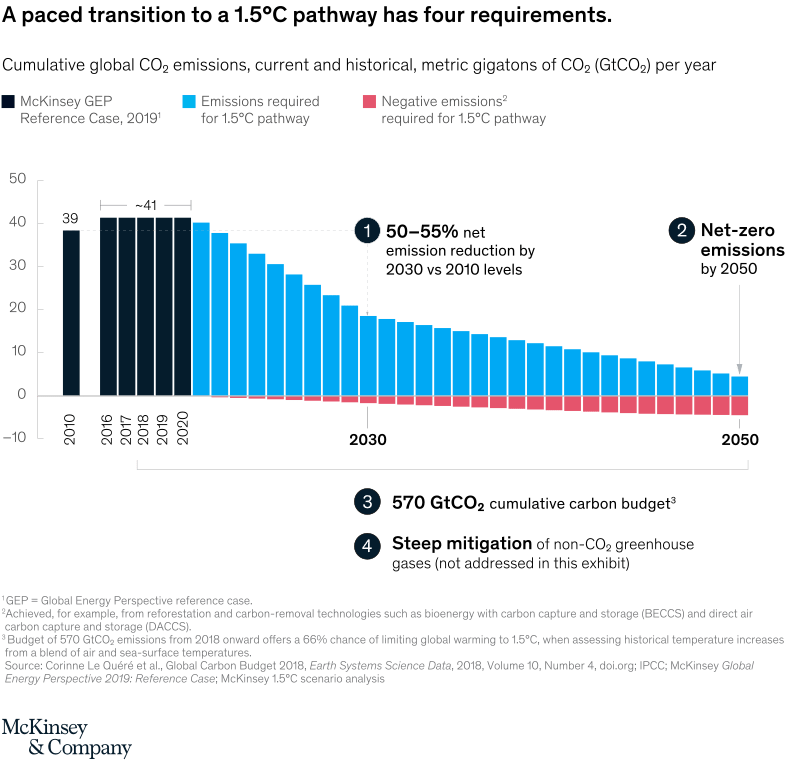
\includegraphics[width=\textwidth]{figures/pathway.png}
    \caption{Projected pathway of carbon emissions reduction required to reach the 1.5-degree goal (Source: McKinsey \& Co., \textit{Climate math: What a 1.5-degree pathway would take})}
\end{figure}
\begin{figure}[ht!]
    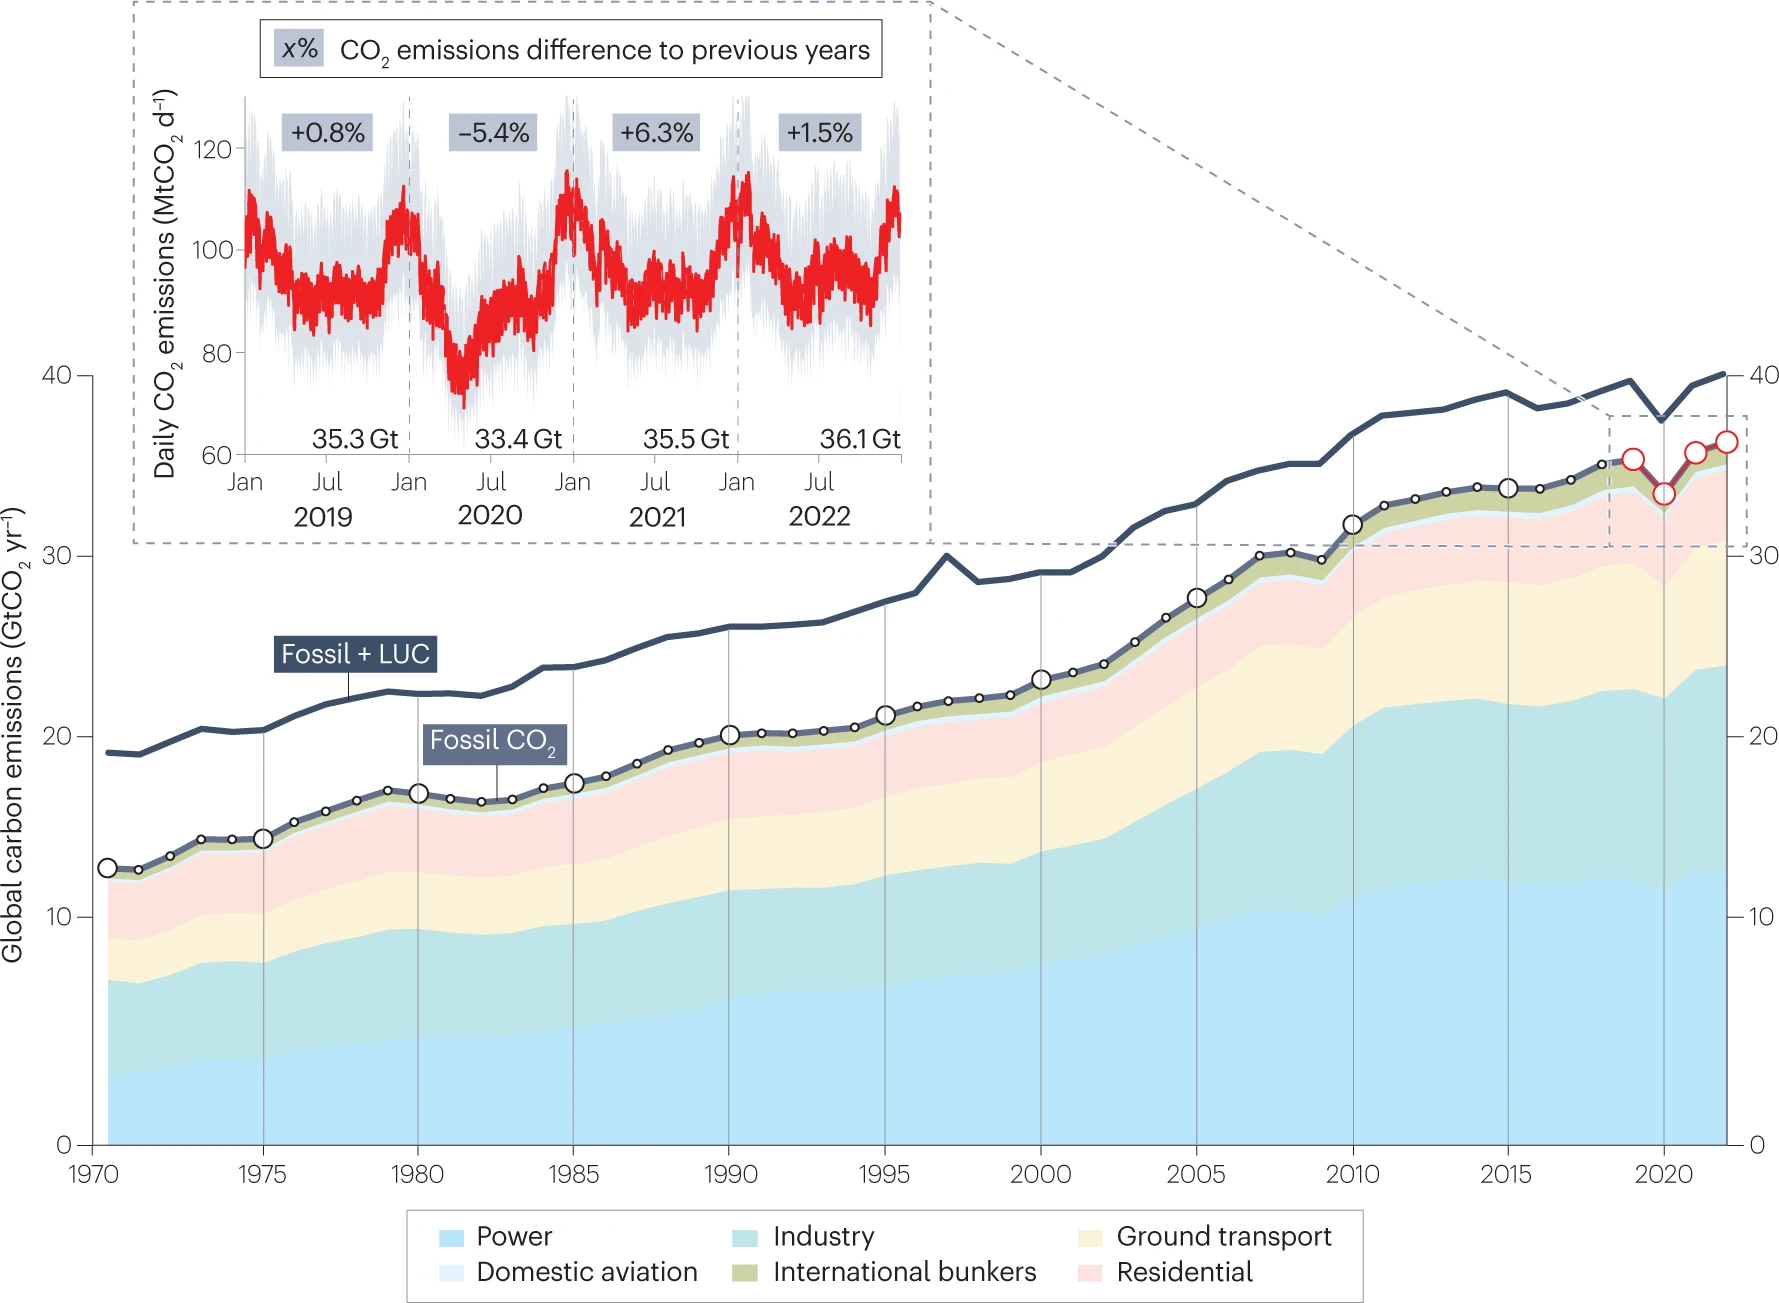
\includegraphics[width=\textwidth]{figures/emissions.png}
    \caption{Actual global carbon dioxide emissions per year from 1900 to 2022 (Source: Liu et al. (2023), \textit{Monitoring global carbon emissions in 2022)}}
\end{figure}

\chapter{Learning effects of DAC}
Learning effects (sometimes called “learning-by-doing”) refer to the phenomenon that individuals or organizations become more efficient or effective at a task over time as they gain experience and knowledge, which can result in significant cost decreases.
This effect was first described by \textcite{Wright1936FactorsAirplanes} in the manufacture of aircraft. He observed that with each doubling of the quantity of aircraft produced, the cost per unit dropped to about 80\% of the previous cost. Since then, learning effects have been observed in a number of manufacturing processes, most prominently in the manufacture of solar photovoltaic modules. Between 2010 and 2020, the cost of solar PV decreased by a factor of five, from approximately 4700 USD/kW to below 900 USD/kW, while the installed capacity increased from 222GW to 1448GW globally. Similar effects, although not of the same magnitude, were observed for wind turbines \parencite{Shrestha2022LearningDeployment}. Mathematically, the experience curve that represents the relationship between the increase in quantity and the reduction in cost is described by \begin{equation} {cost_{new} = cost_{old}*\left( \frac{quantity_{new}}{quantity_{old}} \right)^{-b}} \end{equation} where b is defined as \begin{equation} -b = \frac{\log{PR}}{\log{2}} \end{equation} with PR being the progression ratio, that is, the percentage of the original cost remaining after doubling the quantity \parencite{Fasihi2019Techno-economicPlants}.\\
The literature expects similar learning effects to occur for DAC, based on the similarity of DAC module manufacturing and solar PV module manufacturing. The graph below illustrates possible price decreases, starting with a cost of 600 USD/t CO\textsubscript{2} for an initial 1Mt/y DAC plant. If a 20\% learning rate, that is, an 80\% progress ratio, can be achieved, the cost of DAC would decrease to below 100 USD after the deployment of 260 Mt/y. If an even higher learning rate of 30\%, similar to solar PV, is assumed, this point would be reached at only 33 Mt/y. Using the integral of the experience curve, the necessary investment can be calculated. For a 20\% learning curve, an investment of 37.5 billion USD is required to deploy 260 Mt/y, while for a 30\% learning curve, an investment of 5.5 billion USD would be sufficient to deploy 33 Mt/y.

\begin{figure}[ht!]
    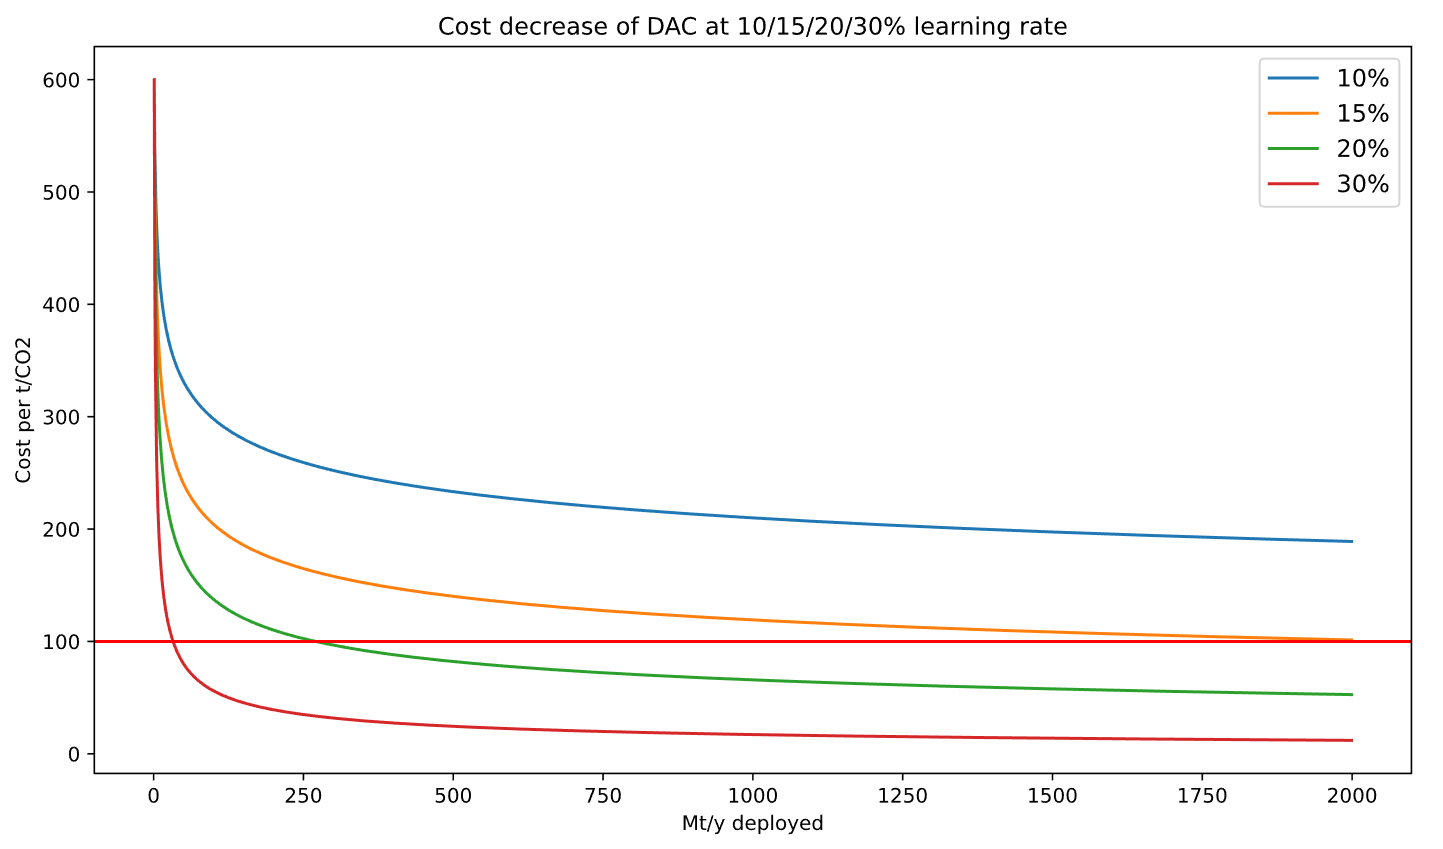
\includegraphics[width=\textwidth]{figures/dac_learning.png}
    \caption{The colored curves show the possible price decreases at different learning rates. The red horizontal line represents the 100 USD/t threshold that must be reached to make DAC economically viable.}
\end{figure}
\newpage
\noindent From this figure it can be concluded that the learning rate will have a significant impact on the future of DAC technology. If a high learning rate is realized, DAC will become relatively cheap rather quickly as commercial deployment progresses. However, if only a low learning rate is observed, DAC may stay prohibitively expensive for the foreseeable future.

\chapter{Overview of potential and cost estimates}
 \mbox{} \begin{center}
    \begin{sideways}%[htbp]
    \captionsetup{margin=0cm}
         \begin{minipage}{1.2\linewidth}
            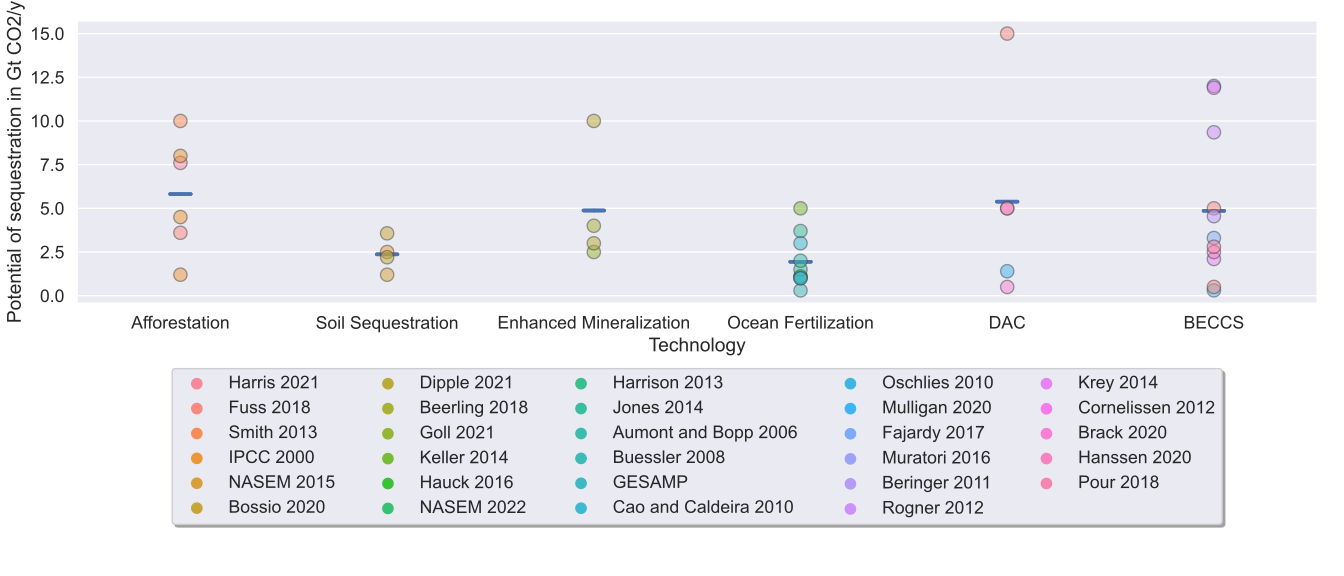
\includegraphics[width=550pt, keepaspectratio]{figures/potential.png}
            \captionof{figure}{Overview of the potential of CDR approaches mentioned in literature. The blue lines represent the average values.}
         \vspace{0.2cm}
         \label{fig:xx}
         \end{minipage}
    \end{sideways}
    \end{center}

\begin{sidewaysfigure}
\captionsetup{margin=3.5cm}
    \centering
    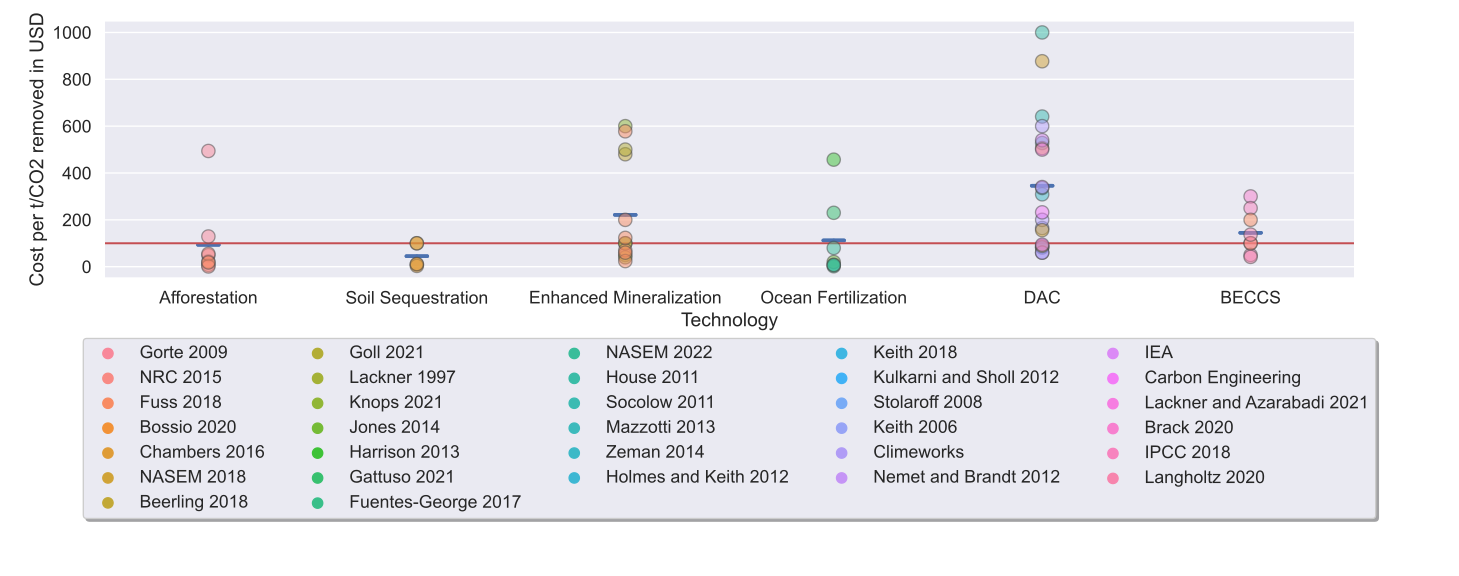
\includegraphics[width=600pt]{figures/cost.png}
    \caption{Overview of the cost of CDR approaches mentioned in literature. The blue lines represent the average values. The red line represents the 100 USD threshold.}
    \label{fig:awesome_image}
\end{sidewaysfigure}

\nocite{House2011EconomicAir, Aumont2006GlobalizingStudies, Buesseler2008OceanUncertainty, Cao2010ImportanceChange, Oschlies2010ClimateApprentice, Beringer2011BioenergyConstraints, Rogner2012EnergyPotentials, Krey2014GlobalReview, Cornelissen2012TheSystem}
\nocite{Cornelissen2012TheSystem, Mazzotti2013DirectContactor, Socolow2011DirectAffairs, Zeman2014ReducingCO2, Nemet2011WillingnessCapture, Kulkarni2012AnalysisAir, Stolaroff2008CarbonSpray}
\nocite{McKinsey2020ClimateTake, Liu2023Monitoring2022}